\documentclass[10pt,twocolumn,letterpaper]{article}

%%%%%%%%% PAPER TYPE  - PLEASE UPDATE FOR FINAL VERSION
\usepackage[review,applications]{wacv}      % To produce the REVIEW version
%\usepackage[applications]{wacv}            % To produce the CAMERA-READY version
%\usepackage[pagenumbers,applications]{wacv} % To force page numbers

\usepackage{microtype}
\usepackage{multirow}

% Corruption / config identifiers, so a name in prose is visibly the same
% token as the one in the released code.
\newcommand{\cfd}{\texttt}

% Bootstrap interval, typeset small under the point estimate it belongs to.
\newcommand{\ci}[2]{{\scriptsize [#1,\,#2]}}

\renewcommand{\topfraction}{0.9}
\renewcommand{\textfraction}{0.07}
\setcounter{topnumber}{3}


% Support for included graphics in the CVF style.
\definecolor{wacvblue}{rgb}{0.21, 0.49, 0.74}
\usepackage[pagebackref,breaklinks,colorlinks,allcolors=wacvblue]{hyperref}

\def\wacvPaperID{*****} % *** Enter the CV4EO Paper ID here
\def\confName{CV4EO}
\def\confYear{2027}

\title{AegisBench: Benchmarking Aerial Person Detection Under\\
Physically Modelled Disaster Conditions}

\author{First Author\\
Institution1\\
Institution1 address\\
{\tt\small firstauthor@i1.org}
% For a paper whose authors are all at the same institution,
% omit the following lines up until the closing ``}''.
% Additional authors and addresses can be added with ``\and'',
% just like the second author.
% To save space, use either the email address or home page, not both
\and
Second Author\\
Institution2\\
First line of institution2 address\\
{\tt\small secondauthor@i2.org}
}

\begin{document}
\maketitle

\begin{abstract}
Aerial person detection supports search and rescue after floods,
wildfires, storms, and at night, yet the benchmarks used to validate it
were collected in calm, clear, well-lit conditions. The operating
conditions that trigger a deployment are precisely the ones that have
never been measured. We present AegisBench, an evaluation benchmark that
places aerial search-and-rescue person detection under nine physically
modelled visual corruptions spanning four disaster families, each at
three severities calibrated against a declared, machine-verified image
statistic. Corruptions are derived from documented atmospheric optics,
including the Koschmieder scattering model for smoke and dust and a
linear-domain photometric model for low light, rather than from generic
image filters. We evaluate three architecturally distinct detectors
across 168 conditions on two datasets spanning the high- and
low-altitude capture regimes, scoring every model with one shared
evaluator at operating points frozen on clean validation data, as a
fielded system would be. Degradation is highly uneven and does not
transfer across capture regimes: heavy rain costs roughly 3.6 points of
recall at the highest severity on one dataset while ranking among the
most damaging corruptions on the other. Low light is universal and
catastrophic, driving recall to exactly zero for all three architectures
on both datasets, with bootstrap confidence intervals degenerate at
$[0.000, 0.000]$; a threshold-independent mAP analysis confirms the
detections are absent rather than below threshold, a three-seed repeat
reproduces the zero exactly, and a check against real night drone
imagery reproduces the collapse. Surviving detections remain accurately
localised, so the failure mode is a detector going blind rather than
mislocalising, which is the mode least visible to a human reviewing the
feed. Finally, we show the collapse is addressable but not free:
fine-tuning on low-light severities 1 and 2 alone lifts severity-3
recall from exactly zero to 0.059--0.188 at a held-out severity, and the
cost to the other eight corruptions is architecture-dependent rather
than uniform, ranging from a net gain to a mean loss of 4.3 points. We
release the corruption engine, the evaluation pipeline, and per-condition
results with intervals for all 168 conditions.
\end{abstract}

\section{Introduction}
\label{sec:intro}

Uncrewed aerial imagery is now a routine instrument for wide-area search
and rescue, and automated person detection is what makes reviewing that
coverage tractable. Speed dominates outcomes: incident data show most
missing subjects are located within the first day, with recovery odds
declining as search time lengthens~\cite{koester2008lost}. A detector
that misses a person in frame is not a benign error.

The two standard benchmarks for this task, HERIDAL~\cite{bozic2019heridal}
and SARD~\cite{sambolek2021sard}, both report strong accuracy, and both
were collected in calm, clear, well-lit conditions. Real missions are
launched because something has gone wrong: after a flood, during a
wildfire, in a storm, or at night. No existing benchmark systematically
measures how these detectors behave under the atmospheric conditions
that trigger their deployment, so the gap between benchmarked accuracy
and operational reliability is, at present, unmeasured.

This gap is unusually tractable in Earth observation, because the
relevant conditions are physically characterisable. Atmospheric
scattering, sediment-laden water, rain, and photon-limited imaging all
have established optical models in the remote-sensing and vision
literature~\cite{koschmieder1924theorie,narasimhan2002vision,garg2007rain,chen2018dark}.
Rather than argue that the evaluation is missing, we build it from those
models.

AegisBench applies nine physically modelled corruptions across four
disaster families to the HERIDAL and SARD test sets and evaluates three
architecturally distinct detectors over all resulting conditions. Three
choices make the result an evaluation protocol rather than a
demonstration. Each corruption is derived from a documented optical
model of a named disaster condition, so a result maps onto an operating
condition a responder can recognise. Each severity is calibrated against
a declared, machine-verified image statistic rather than chosen by eye,
so severity claims are falsifiable. Every detector's confidence
threshold is selected once on clean validation data and frozen across
all corrupted conditions, matching how a system is fielded rather than a
best case unavailable mid-mission.

What the benchmark then measures is not a uniform loss of accuracy. It
is a set of failures that differ by condition, by capture regime and by
architecture, with one of them sitting at the absolute floor. We report
the measurement, establish that the floor is not an artefact of
thresholds, seeds or the corruption model, and then show what it takes
to move it.

\paragraph{Contributions.}
\begin{itemize}\itemsep1pt \parskip0pt \topsep2pt
\item A physically grounded corruption benchmark for aerial
search-and-rescue person detection: nine corruptions, four disaster
families, three calibrated severities, bit-reproducible from the source
datasets without redistributing imagery
(Section~\ref{sec:benchmark}).
\item A 168-condition evaluation of three architecturally distinct
detectors under one shared evaluator at frozen operating points, with
bootstrap intervals on every condition, showing that degradation is
uneven, that it does not transfer between capture regimes, and that
low light drives all three architectures to exactly zero recall
(Section~\ref{sec:results}).
\item Three independent checks that the zero is real rather than an
artefact: a threshold-independent mAP analysis, a three-seed repeat, and
an evaluation on real night drone imagery at the frozen operating point
(Sections~\ref{sec:results} and~\ref{sec:mitigation}).
\item A localisation analysis showing the failure is a loss of
detections rather than of box placement, which identifies the failure as
silent and locates where a mitigation must act
(Section~\ref{sec:results}).
\item A mitigation study that lifts severity-3 low-light recall off the
floor by training only on severities 1 and 2, and a measurement of what
that costs on the other eight corruptions, which turns out to be
architecture-dependent rather than a single robustness tax
(Section~\ref{sec:mitigation}).
\end{itemize}

\section{Related Work}
\label{sec:related}

\paragraph{Aerial person detection for search and rescue.}
HERIDAL~\cite{bozic2019heridal} and SARD~\cite{sambolek2021sard} are the
two datasets this task is normally validated on. They differ in capture
regime, HERIDAL at high altitude over wilderness terrain with very small
subjects and SARD at lower altitude with larger relative object size,
and together they cover most of what the literature reports. Both were
collected in clear daytime conditions, and both are evaluated that way.
VisDrone~\cite{zhu2022visdrone} is broader in scene content and includes
genuine night frames, but it is urban and artificially lit, and person
annotations there describe a different operating context than wilderness
search. We use it only as an independent check, never for training,
calibration or threshold selection.

\paragraph{Corruption robustness benchmarks.}
ImageNet-C~\cite{hendrycks2019imagenetc} established the pattern this
work follows: hold the dataset fixed, apply a fixed corruption ladder,
and report accuracy per condition rather than as a single number.
Michaelis \etal~\cite{michaelis2019benchmarking} carried the protocol to
detection and showed stylisation-based augmentation recovers a
substantial part of the loss, which is the independent precedent our
mitigation arm draws on. These benchmarks are built from generic image
operations chosen for breadth. That is the right choice for a general
recognition benchmark and the wrong one here, because a responder
selecting a system for a night flood mission needs a number attached to
a named condition, not to a filter. Foggy Cityscapes~\cite{sakaridis2018foggy}
is the closest precedent for the alternative: it synthesises fog from
the Koschmieder model on real imagery with depth, and demonstrates that
a physically derived corruption applied to real scenes supports
controlled attribution. AegisBench extends that stance from one
condition in one domain to nine conditions across four disaster families
in aerial Earth observation, and adds a declared per-corruption
calibration statistic so that severity claims are falsifiable rather
than stipulated.

\paragraph{Optical models of degraded imaging.}
The corruption implementations are not new physics. Atmospheric
scattering follows Koschmieder~\cite{koschmieder1924theorie} in the form
standardised for vision by Narasimhan and
Nayar~\cite{narasimhan2002vision}; rain streaks follow the additive
directional model of Garg and Nayar~\cite{garg2007rain}; low light
follows the linear-domain photometric account of photon-limited capture
used by Chen \etal~\cite{chen2018dark}, including the signal-dependent
noise that dominates as light falls. The contribution is not the models
but their use as a calibrated, reproducible evaluation axis for a
safety-of-life aerial task, together with the parameter ranges,
calibration statistics and seeding discipline that make a severity mean
the same thing across capture regimes.

\paragraph{What is missing.}
Across these lines of work, robustness for aerial search and rescue is
reported either under clear conditions or under generic distortions, and
almost always at a tuned operating point. None of the three gaps is
exotic: what is absent is a benchmark that names the disaster condition,
calibrates its severity, and scores every architecture through one
evaluator at a threshold a fielded system could actually have chosen in
advance. That combination is what AegisBench supplies, and it is what
makes the low-light result in Section~\ref{sec:results} interpretable as
an operational finding rather than a tuning artefact.

\section{Benchmark and Protocol}
\label{sec:benchmark}

\subsection{Corruption taxonomy}

Nine corruptions are grouped into four disaster families: flood
(\cfd{water\_glare}, \cfd{turbidity\_cast}, \cfd{inundation}), wildfire
(\cfd{smoke\_haze}, \cfd{fire\_warm\_tint}), storm (\cfd{rain\_streaks},
\cfd{motion\_blur}, \cfd{low\_light}), and earthquake and post-disaster
(\cfd{dust\_haze}); see Figure~\ref{fig:taxonomy}. Grouping by disaster
family rather than by distortion type is deliberate, so a result reads
as ``this system loses $X$ of its detections in wildfire smoke'' rather
than as a filter name. With three severities each plus the clean
condition, one model on one dataset is measured over 28 conditions, and
the full study over 168.

\subsection{Physical models}

The three haze-family corruptions are built on the Koschmieder
atmospheric scattering model~\cite{koschmieder1924theorie,narasimhan2002vision},
$I = Jt + A(1-t)$, with $J$ the clear-scene radiance, $A$ the
atmospheric light and $t$ the transmission map. \cfd{smoke\_haze} and
\cfd{dust\_haze} differ principally in the chromaticity of $A$, neutral
grey for combustion aerosol against a brown mineral airlight for
suspended particulate, a distinction verified by a unit test on the
red-to-blue channel ratio. Sediment-laden water is not a scattering
process, so the flood family is modelled separately: \cfd{turbidity\_cast}
blends toward a mud chromaticity with contrast compression toward the
scene mean and saturation loss, \cfd{water\_glare} adds thresholded
specular glint cores with a Gaussian bloom halo, and \cfd{inundation}
composites semi-transparent standing water over part of the scene with a
ripple displacement of the submerged content.

\cfd{low\_light} is modelled in the linear photometric
domain~\cite{chen2018dark}. The image is linearised, scaled by a photon
gain, given a twilight blue shift, and returned through the transfer
curve with signal-dependent shot noise and signal-independent read noise
whose relative magnitude grows as light falls. This matters for what the
benchmark measures: the severities are not a gamma darkening but a loss
of photons, so contrast and signal-to-noise degrade together the way
they do on a real sensor at dusk. The three severities apply linear
gains of 0.33, 0.13 and 0.045, which is an exposure loss of roughly 1.6,
2.9 and 4.5 stops, with the read-noise floor rising from 0.010 to 0.028
across the ladder. Severity 3 is therefore late dusk rather than
darkness, which is worth keeping in mind against the results that
follow. \cfd{rain\_streaks} follows the additive
directional-streak model of Garg and Nayar~\cite{garg2007rain}, and
\cfd{motion\_blur} applies a directional kernel scaled to image size.

\subsection{Calibration}

Each corruption declares a measurable image statistic that must move
monotonically across its three severities, verified on a fixed random
20-image subset held constant across all corruptions so that comparisons
are made against identical scene content. Eight of nine pass directly.
\cfd{rain\_streaks} does not: its declared statistic, streak density,
has no closed-form image measure, and the substituted edge-strength
proxy is confounded because added streaks raise measured edge strength
while the veil blur suppresses it. Its severity is instead defined by
monotonically increasing generation parameters (streaks per megapixel,
streak length and veil intensity) and verified by visual audit;
downstream recall degrades in the expected direction regardless,
independent evidence that the corruption intensifies even though this
one proxy does not track it. We report this rather than substituting a
statistic chosen after the fact for passing.

The statistic calibrates each ladder \emph{within} a corruption; it is
not a cross-corruption difficulty normaliser, and two corruptions
matched on the same statistic are not expected to be equally damaging.
\cfd{smoke\_haze} and \cfd{dust\_haze} illustrate this directly: they
reach nearly identical RMS contrast at every severity (0.0475 versus
0.0489 at severity 3) yet differ 6.7-fold in cost
(Table~\ref{tab:spectrum} and Table~\ref{tab:family}), showing detection
difficulty here is not reducible to global contrast reduction alone. We
do not isolate which remaining difference, airlight chromaticity,
transmission-field granularity or added grain, carries the effect, and
flag it as an open question.

\subsection{Determinism and reproducibility}

Pixel-unit parameters are specified per 1000 pixels of the longer image
side and scaled at runtime, so a severity means the same thing across
capture regimes. Corruptions are appearance-only, leaving clean
ground-truth boxes exactly valid. Every stochastic element is seeded
from a SHA-256 stable hash of image identity, corruption, severity and
global seed, independent of platform, so the corrupted benchmark
regenerates bit-identically anywhere. We redistribute no imagery; the
released code and parameters reproduce it from the source datasets,
which preserves both licences and the ability to audit what was applied.

\subsection{Datasets and detectors}

HERIDAL~\cite{bozic2019heridal} is captured at high altitude over
wilderness terrain at $4000 \times 3000$, and its test split holds 101
images with 337 annotated persons. The evaluated SARD~\cite{sambolek2021sard}
copy is a re-export at $640 \times 640$, captured lower with larger
relative object size, and its test split holds 862 images with 1097
persons. The two therefore span the high- and low-altitude capture
regimes, which is what makes the transfer question in
Section~\ref{sec:results} answerable at all.

Both datasets pass through the same tiling pipeline, 1024-pixel tiles at
256-pixel overlap, chosen so the overlap exceeds the largest person box.
On HERIDAL this genuinely tiles each frame into 20; on SARD the source
frames are smaller than the tile, so each passes through as a single
full-frame tile. Running one protocol on both is deliberate, since it
removes an experimenter degree of freedom when comparing capture
regimes, and we state the differing behaviour rather than hiding it.
Predictions are mapped back and evaluated against full-resolution ground
truth after class-agnostic non-maximum suppression.

We fine-tune three architecturally distinct detectors: Faster
R-CNN~\cite{ren2015fasterrcnn} (two-stage CNN),
YOLOv11~\cite{ultralytics2024yolo11} (single-stage CNN) and
RT-DETR~\cite{zhao2024rtdetr} (transformer), one run per model per
dataset, all at 1024-pixel input on a single 8\,GB consumer GPU. The
hardware budget is worth stating because it means the benchmark is
reproducible without cluster access. Training is the standard recipe for
each framework rather than a tuned one, since the object of study is the
evaluation axis and not a new detector.

\subsection{Evaluation protocol}

Thresholds are selected once per model per dataset by maximising F1 on
clean validation data and frozen across all 28 conditions for that
model; corrupted data enters neither training nor threshold selection.
This is the single most consequential protocol choice in the paper. A
threshold retuned per condition would report the best case available to
an oracle, which is not a case a fielded system has access to mid-mission,
and it would hide exactly the failure we find.

All architectures are scored by one evaluator, greedy score-ordered
matching at IoU $\geq 0.5$, so no model is scored by its own framework's
metric. Corruptions are applied to the full frame before tiling, since
haze gradients and flood masks are spatially coherent across a scene and
applying them per tile would introduce seams the physics does not
produce. Degradation is reported relative to each model's own clean
score, since the datasets do not share a difficulty floor. Confidence
intervals are bootstrap percentile over 1000 resamples of the test set
by image~\cite{efron1993bootstrap}, resampling images rather than
instances so that the interval reflects scene-level variability.

\begin{figure}[t]
\centering
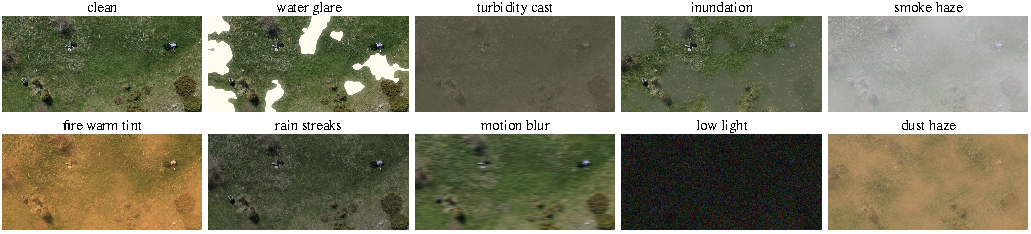
\includegraphics[width=\columnwidth]{figures/taxonomy_s3.pdf}
\caption{The nine corruptions at severity 3 on a cropped HERIDAL frame.
Each models a documented optical signature of a disaster environment
rather than a generic distortion.}
\label{fig:taxonomy}
\end{figure}

\section{Results}
\label{sec:results}

Clean recall is 0.745--0.792 on HERIDAL and 0.879--0.891 on SARD,
consistent with SARD's lower-altitude capture and larger relative object
size. Every number reported below is recall at that model's own frozen
operating point unless stated otherwise, and every condition carries a
bootstrap interval in the released per-condition table.

\subsection{Degradation is uneven and does not transfer}

At matched severity 3 on SARD, YOLOv11 recall ranges from 0.855 under
\cfd{rain\_streaks}, a 3.6-point drop from its 0.891 clean baseline, to
exactly 0.000 under \cfd{low\_light} (Table~\ref{tab:spectrum}). That is
the whole span of the outcome space inside one dataset, one model and
one severity level, which is the first reason a single averaged
robustness score is the wrong summary for this task.

The same corruption also behaves differently across capture regimes.
\cfd{rain\_streaks} is the mildest corruption on SARD for all three
detectors, yet on HERIDAL it sits among the most damaging, where the
storm-family relative recall drop reaches 0.784--0.874. We do not
isolate which property of the capture regime produces the reversal, and
the obvious candidate is not straightforward: by COCO area bands both
test sets are dominated by medium-sized instances (327 of 337 on
HERIDAL, 789 of 1097 on SARD), so absolute subject size alone does not
explain it. What the result does establish is the consequence: a
robustness number measured at one altitude does not transfer to another,
which matters directly for anyone selecting a system against a mission
profile.

Table~\ref{tab:family} aggregates relative recall drop by disaster
family across all three detectors and both datasets. Flood is the
mildest family without exception, the one ordering fully consistent
across the study. Storm is worst on HERIDAL, pulled up by the low-light
collapse, and earthquake is worst on SARD. Figure~\ref{fig:heatmap}
shows the same pattern per corruption, with the \cfd{low\_light} row
saturating for all three architectures.

\begin{table}[t]
\centering\small
\setlength{\tabcolsep}{3pt}
\caption{Mean relative recall drop by disaster family, averaged over
severities. Flood is mildest on both datasets for every model; storm is
worst on HERIDAL, earthquake worst on SARD.}
\label{tab:family}
\begin{tabular}{lccc}
\toprule
Family & F.\ R-CNN & RT-DETR & YOLOv11 \\
\midrule
\multicolumn{4}{l}{\emph{HERIDAL}} \\
Storm      & 0.784 & 0.874 & 0.829 \\
Earthquake & 0.534 & 0.568 & 0.571 \\
Wildfire   & 0.335 & 0.459 & 0.405 \\
Flood      & 0.301 & 0.231 & 0.246 \\
\midrule
\multicolumn{4}{l}{\emph{SARD}} \\
Earthquake & 0.481 & 0.630 & 0.624 \\
Storm      & 0.401 & 0.440 & 0.413 \\
Wildfire   & 0.327 & 0.451 & 0.445 \\
Flood      & 0.264 & 0.293 & 0.252 \\
\bottomrule
\end{tabular}
\end{table}

\begin{figure}[t]
\centering
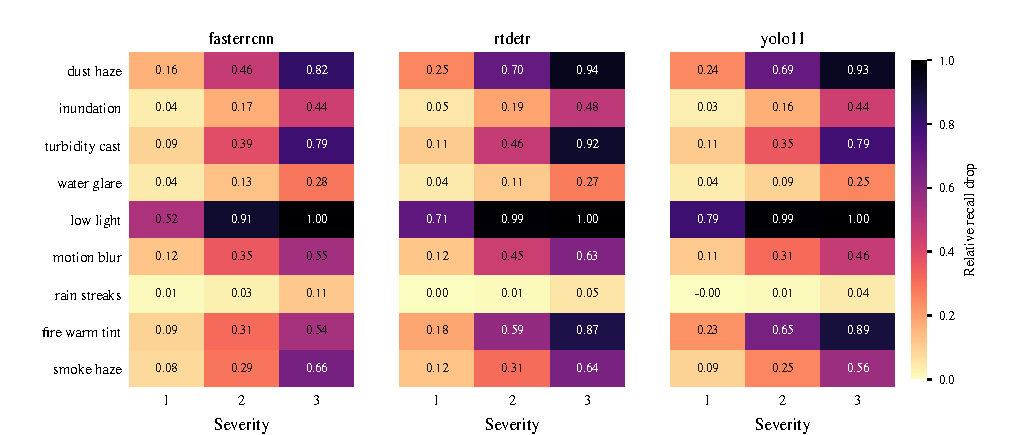
\includegraphics[width=\columnwidth]{figures/heatmap_sard.pdf}
\caption{Relative recall drop, (clean$-$corrupted)/clean, for each
detector on SARD. Rows grouped by disaster family. The
\cfd{low\_light} row saturates for all three architectures.}
\label{fig:heatmap}
\end{figure}

\subsection{Low light collapses detection across all architectures}

By severity 3, recall is exactly 0.000 for all three architectures on
both HERIDAL ($n{=}101$ images, 337 persons) and SARD ($n{=}862$ images,
1097 persons), and every one of 1000 bootstrap resamples agrees, so the
interval is degenerate at $[0.000,0.000]$ (Table~\ref{tab:lowlight}).
Not one annotated person is recovered anywhere in either test set. A
two-stage CNN, a single-stage CNN and a transformer sit at the same
floor, which rules out an architecture-specific explanation, and the
condition producing it is an exposure loss of about 4.5 stops rather
than true darkness.

\paragraph{It is not the threshold.} The natural objection is that a
frozen-threshold zero reflects a badly placed operating point rather
than a failure to detect. mAP$_{50}$ settles it, since it scans every
threshold: on HERIDAL at severity~1, RT-DETR's mAP$_{50}$ falls from
0.835 clean to 0.001, YOLOv11's from 0.803 to 0.064 and Faster R-CNN's
from 0.785 to 0.537, in lockstep with frozen-threshold recall. Were this
a calibration artefact, mAP would stay high while recall fell; it does
not. The same point holds across models rather than only within one:
Faster R-CNN is consistently the most robust wherever any model retains
recall, despite carrying the strictest frozen threshold (0.99 on
HERIDAL, 0.96 on SARD), which rules out threshold strictness as the
explanation for the ordering.

\paragraph{It is not the seed.} A single training run per model leaves
open that the zero is a property of one unlucky checkpoint. We repeated
the SARD YOLOv11 run at two further seeds, 42 and 123, each trained and
threshold-selected independently under the identical protocol, and
re-swept the low-light ladder (Table~\ref{tab:seeds}). Clean recall
moves only between 0.874 and 0.891 and the independently selected
threshold moves only between 0.30 and 0.35, so the three runs are
comparable. Severity-1 recall varies materially, from 0.184 to 0.234,
which is worth noting as the honest scale of run-to-run variation on
this ladder. Severity 3 does not vary at all: all three seeds return
exactly 0.000 with degenerate intervals. The collapse is a property of
the condition, not of a checkpoint.

\begin{table}[t]
\centering\small
\setlength{\tabcolsep}{3.5pt}
\caption{Multi-seed repeat, YOLOv11 on SARD, under \cfd{low\_light}.
Each seed is trained and threshold-selected independently. Bootstrap
95\% intervals over 1000 resamples in brackets. Severity-1 recall varies
across seeds; severity 3 is exactly zero for all three.}
\label{tab:seeds}
\begin{tabular}{lccc}
\toprule
 & Seed 17 & Seed 42 & Seed 123 \\
\midrule
Threshold & 0.30 & 0.35 & 0.30 \\
Clean     & 0.891 & 0.874 & 0.885 \\
\midrule
s1 & 0.184 & 0.200 & 0.234 \\
   & \ci{0.154}{0.213} & \ci{0.170}{0.229} & \ci{0.207}{0.265} \\
s2 & 0.007 & 0.008 & 0.021 \\
   & \ci{0.003}{0.013} & \ci{0.003}{0.014} & \ci{0.012}{0.029} \\
s3 & \textbf{0.000} & \textbf{0.000} & \textbf{0.000} \\
   & \ci{0.000}{0.000} & \ci{0.000}{0.000} & \ci{0.000}{0.000} \\
\bottomrule
\end{tabular}
\end{table}

\paragraph{It is not only the corruption model.} Because the corruption
is synthetic, we evaluated the SARD-trained YOLOv11, at its frozen
operating point and without retraining, on 40 real nighttime images from
VisDrone~\cite{zhu2022visdrone}, held out from training, calibration and
threshold selection. Recall was 0.016, close to the floor the synthetic
corruption reaches at severity 3. The settings are not equivalent, as
VisDrone night scenes are urban and artificially lit whereas
search-and-rescue imagery is unlit terrain, and 40 images is a spot
check rather than a benchmark. Read narrowly, it indicates the failure
is not an artefact of the corruption model. We state the weakness of
this check plainly in Section~\ref{sec:discussion} rather than resting
the claim on it.

Taken together, the three checks close off the three ways this result
could have been an artefact of our own setup. What remains is a property
of photon-limited aerial imagery and the detectors as trained.

\subsection{The failure is a loss of detections, not of localisation}

For instances detected in both the clean and corrupted conditions, we
measure the IoU between the two predicted boxes, a scale-normalised
centre shift, and the drop in box-versus-ground-truth fit. Restricting
to commonly detected instances keeps the metric unconfounded by recall:
it asks whether a surviving detection stayed planted on the person,
which is a different question from whether the person was found at all.

Figure~\ref{fig:decoupling} plots recall against localisation stability
for YOLOv11 on SARD, one point per corruption and severity, with both
axes spanning the full unit range. Stability declines only from 0.98 to
0.78 across the entire severity range while recall falls from 0.89 to
0.00, and the count of commonly detected instances tracks recall exactly
(\cfd{low\_light}: 202, then 8, then 0). Recall sweeps nearly the whole
unit range while stability stays in a narrow band near the top, never
below 0.78 even where almost every detection is lost.

The dominant failure mode is therefore a detection disappearing, not a
box drifting off the person. This matters operationally: a mislocalised
box is a visible error an operator can catch, whereas a frame with no
detections is indistinguishable from a correctly searched empty frame.
Under the conditions measured here, these systems fail silently, in the
direction that resembles task completion. It also says where a
mitigation should aim, at sensitivity rather than at localisation, which
is the design the next section tests.

\begin{figure}[t]
\centering
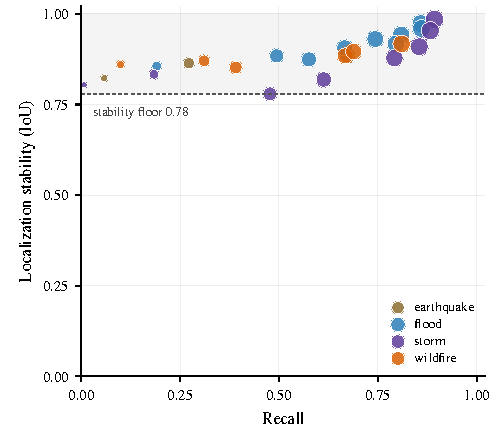
\includegraphics[width=0.85\columnwidth]{figures/decoupling_sard_yolo11.pdf}
\caption{Recall against localisation stability, YOLOv11 on SARD, one
point per corruption and severity. Points sweep the entire recall range
while remaining in a narrow band near the top of the stability axis.}
\label{fig:decoupling}
\end{figure}

\begin{table}[t]
\centering\small
\setlength{\tabcolsep}{4pt}
\caption{Recall by corruption and severity, YOLOv11 on SARD, at the
frozen operating point of 0.30. Clean baseline 0.891. The span within
this single table, 0.855 to 0.000 at severity 3, is why an averaged
robustness score is the wrong summary.}
\label{tab:spectrum}
\begin{tabular}{llccc}
\toprule
Corruption & Family & s1 & s2 & s3 \\
\midrule
\cfd{rain\_streaks}    & Storm      & 0.893 & 0.882 & \textbf{0.855} \\
\cfd{water\_glare}     & Flood      & 0.859 & 0.809 & 0.666 \\
\cfd{inundation}       & Flood      & 0.861 & 0.744 & 0.495 \\
\cfd{motion\_blur}     & Storm      & 0.792 & 0.613 & 0.478 \\
\cfd{smoke\_haze}      & Wildfire   & 0.810 & 0.667 & 0.391 \\
\cfd{turbidity\_cast}  & Flood      & 0.796 & 0.575 & 0.191 \\
\cfd{fire\_warm\_tint} & Wildfire   & 0.688 & 0.310 & 0.099 \\
\cfd{dust\_haze}       & Earthquake & 0.674 & 0.273 & 0.058 \\
\cfd{low\_light}       & Storm      & 0.184 & 0.007 & \textbf{0.000} \\
\bottomrule
\end{tabular}
\end{table}

\begin{table}[t]
\centering\small
\setlength{\tabcolsep}{3pt}
\caption{Recall under \cfd{low\_light} at each model's frozen operating
point, with clean recall for reference. Once recall is exactly zero on
the full test set every bootstrap resample returns zero, so the interval
is degenerate by construction.}
\label{tab:lowlight}
\begin{tabular}{lccccc}
\toprule
Model & Thr. & Clean & s1 & s2 & s3 \\
\midrule
\multicolumn{6}{l}{\emph{HERIDAL} (101 images, 337 persons)} \\
Faster R-CNN & 0.99 & 0.745 & 0.451 & 0.110 & \textbf{0.000} \\
YOLOv11      & 0.45 & 0.769 & 0.047 & 0.000 & \textbf{0.000} \\
RT-DETR      & 0.65 & 0.792 & 0.000 & 0.000 & \textbf{0.000} \\
\midrule
\multicolumn{6}{l}{\emph{SARD} (862 images, 1097 persons)} \\
Faster R-CNN & 0.96 & 0.879 & 0.419 & 0.077 & \textbf{0.000} \\
RT-DETR      & 0.60 & 0.888 & 0.260 & 0.013 & \textbf{0.000} \\
YOLOv11      & 0.30 & 0.891 & 0.184 & 0.007 & \textbf{0.000} \\
\bottomrule
\end{tabular}
\end{table}

\section{Moving the Floor: A Mitigation Study}
\label{sec:mitigation}

A benchmark that only reports a failure invites the reading that the
failure is intrinsic. The localisation analysis says otherwise: the
detectors lose sensitivity, not box placement, which is the kind of
deficit training data can address. We test that directly, and we design
the test so that a positive result cannot be an artefact of training on
the condition being scored.

\subsection{Design}

For each of the three SARD detectors we fine-tune the existing clean
checkpoint on training tiles augmented with \cfd{low\_light} at
\textbf{severities 1 and 2 only}. Severity 3, the condition where all
three collapse, is held out of training entirely and is only ever seen
at evaluation. Reporting a recovery at a severity the model was trained
on would measure memorisation of a known condition; holding severity 3
out makes the question generalisation along the ladder, which is the
question a deployment actually faces, since the weather on the night of
a callout is not the weather in the training set.

Three further constraints keep the comparison honest. Validation data
stays clean, enforced by the augmentation script, so the operating point
cannot drift with the augmentation. Each mitigated checkpoint has its
threshold re-selected on its own clean validation data by the same
F1-maximising rule used for every other model in the paper, and then
frozen across all 28 conditions; it does not inherit the baseline's
threshold, because that would score a new model at another model's
operating point. And every mitigated model is re-swept over the full
28-condition grid, not only over low light, so that the cost of the
intervention elsewhere is measured rather than assumed.

\subsection{The collapse is addressable}

Table~\ref{tab:mitigation} gives the result. At the held-out severity 3,
recall moves off the floor for all three architectures: from exactly
0.000 to 0.121 for Faster R-CNN, 0.059 for RT-DETR and 0.188 for
YOLOv11, with bootstrap intervals that exclude zero in every case. At
the trained severities the recovery is much larger, from 0.419 to 0.843,
0.260 to 0.772 and 0.184 to 0.807 at severity 1, and from at most 0.077
to between 0.529 and 0.647 at severity 2.

Two readings are available and we take the conservative one. A
severity-3 recall of 0.059 to 0.188 is not an operational fix; a system
that finds one subject in five at late dusk is still failing. What the
result establishes is narrower and sufficient for the benchmark's
purpose: the zero is not a hard limit of these architectures under
photon-limited capture, it is a data-coverage deficit that responds to
targeted training, and it responds even one full severity step beyond
the training distribution. The benchmark therefore measures something
that can be optimised against, which is the property that makes an
evaluation axis useful rather than merely discouraging.

\begin{table}[t]
\centering\small
\setlength{\tabcolsep}{3pt}
\caption{Low-light mitigation on SARD. Each model is fine-tuned on
severities 1 and 2 only; \textbf{severity 3 is held out of training} and
seen only at evaluation. Thresholds are re-selected on clean validation
data for each mitigated checkpoint and frozen. Bootstrap 95\% intervals
over 1000 resamples for the mitigated models.}
\label{tab:mitigation}
\begin{tabular}{llcccc}
\toprule
Model & & Clean & s1 & s2 & s3 \\
\midrule
\multirow{3}{*}{F.\ R-CNN}
 & before & 0.879 & 0.419 & 0.077 & 0.000 \\
 & after  & 0.900 & 0.843 & 0.641 & \textbf{0.121} \\
 & 95\%   &       & \ci{0.818}{0.865} & \ci{0.612}{0.669} & \ci{0.101}{0.140} \\
\midrule
\multirow{3}{*}{RT-DETR}
 & before & 0.888 & 0.260 & 0.013 & 0.000 \\
 & after  & 0.858 & 0.772 & 0.529 & \textbf{0.059} \\
 & 95\%   &       & \ci{0.745}{0.798} & \ci{0.497}{0.560} & \ci{0.046}{0.073} \\
\midrule
\multirow{3}{*}{YOLOv11}
 & before & 0.891 & 0.184 & 0.007 & 0.000 \\
 & after  & 0.883 & 0.807 & 0.647 & \textbf{0.188} \\
 & 95\%   &       & \ci{0.782}{0.830} & \ci{0.615}{0.678} & \ci{0.168}{0.211} \\
\bottomrule
\end{tabular}
\end{table}

\subsection{What it costs, and why the cost is not one number}

The interesting part is the price. Because each mitigated model was
re-swept over the whole grid, we can measure the change on the eight
corruptions that were never trained on, 24 conditions per model, as well
as on clean data (Table~\ref{tab:tradeoff}).

The result does not resolve into a single robustness tax. Faster R-CNN
improves on average by 3.7 points across the other 24 conditions, gains
2.1 points on clean data, and its worst single regression is 2.5 points,
so nothing degrades by more than the noise band of 3 points that we use
as a reporting cutoff. RT-DETR moves the other way: it loses 4.3 points
on average, regresses by more than 3 points on 17 of 24 conditions, loses
3.0 points on clean data, and its worst case is 11.6 points. YOLOv11 sits
between them, losing 1.9 points on average with 8 of 24 conditions
regressing by more than 3 points.

Because all three arms use the same augmented data, the same held-out
severity, the same threshold-selection rule and the same evaluator, the
spread across them is attributable to architecture rather than to
protocol. We do not claim a mechanism. We note that the transformer
detector, which already carries the largest relative recall drop of the
three in every disaster family on SARD (Table~\ref{tab:family}), is also
the one for which targeted augmentation is most
expensive elsewhere, and that this is precisely the kind of interaction
that a benchmark reporting one averaged robustness number could not
surface. The practical implication for a deployment is that
``augment for the condition you expect'' is sound advice for some
architectures and a regression for others, and which one it is has to be
measured on the full grid rather than inferred.

\begin{table}[t]
\centering\small
\setlength{\tabcolsep}{3pt}
\caption{Cost of low-light augmentation on conditions it was not trained
for: change in recall over the eight other corruptions at three
severities (24 conditions per model), plus clean. Positive is better.
The sign of the mean differs by architecture.}
\label{tab:tradeoff}
\begin{tabular}{lcccc}
\toprule
 & $\Delta$ clean & Mean $\Delta$ & Worst & \#\,worse \\
 &                & (24 cond.)    & $\Delta$ & by $>$0.03 \\
\midrule
F.\ R-CNN & $+0.021$ & $+0.037$ & $-0.025$ & 0/24 \\
YOLOv11   & $-0.007$ & $-0.019$ & $-0.066$ & 8/24 \\
RT-DETR   & $-0.030$ & $-0.043$ & $-0.116$ & 17/24 \\
\bottomrule
\end{tabular}
\end{table}

\subsection{Scope of this study}

The mitigation arm is one augmentation strategy, on one dataset, at one
seed per architecture, targeting one corruption. It is enough to settle
whether the floor is movable and to show that the cost of moving it is
architecture-dependent. It is not enough to recommend a training recipe,
and we do not. The natural extensions, sweeping the augmentation across
the other corruptions, repeating it on HERIDAL, and combining
conditions as a real mission would, are supported by the released
pipeline and are left open.

\section{Discussion}
\label{sec:discussion}

\paragraph{What a responder can take from this.} Three findings are
actionable without any further work. A robustness claim for an aerial
person detector is not portable across altitude, so a number quoted from
one capture regime should not be used to select a system for another.
Low light is not a graded degradation for these detectors but a cliff,
and at roughly 4.5 stops of exposure loss the systems return nothing at
all. And because the failure is a loss of detections rather than
mislocalisation, an empty feed under degraded conditions carries no
information: it is indistinguishable from a correctly searched empty
frame, so it should not be treated as coverage.

\paragraph{Why per-condition reporting is the unit.} Every headline in
this paper is invisible under averaging. The span in
Table~\ref{tab:spectrum} runs from a 3.6-point loss to a total one
inside one model and one severity. The rain reversal between datasets
cancels if the two are pooled. The mitigation trade-off in
Table~\ref{tab:tradeoff} changes sign across architectures. We therefore
release results per condition, per model and per dataset with intervals,
and would encourage the same shape for any robustness result intended to
inform a deployment decision.

\paragraph{Limitations.} Four bound what is claimed here. First, the
corruptions are synthetic, applied to real imagery, following the
ImageNet-C and Foggy Cityscapes
lineage~\cite{hendrycks2019imagenetc,sakaridis2018foggy}; this is what
makes controlled per-condition attribution possible, since disaster
imagery rarely has a matched clean counterpart of the same scene, but it
is also the ceiling of the method. Second, the VisDrone spot check is
40 images and is suggestive rather than a substitute for systematic
validation against real adverse-condition search-and-rescue footage,
which is made harder by how rarely such footage is released: aerial
disaster imagery exists for related tasks such as fire segmentation but
not with person annotations, itself a gap this release may help motivate
closing. Third, we evaluate two datasets and three detectors,
prioritising depth of protocol over breadth of coverage, and the
multi-seed confirmation covers one model on one dataset. Fourth,
corruptions are applied one at a time, whereas a real night flood
presents several at once; the released engine composes them, but we do
not report the combinatorial grid and do not assume the effects are
additive.

\paragraph{Ethics and responsible release.} We use only publicly
available research datasets under their own terms and collect no
human-subjects data. We add no imagery and no annotations of people, and
annotate no identity, biometric or demographic attribute; persons appear
only as generic boxes inherited from the sources. Automated aerial
person detection is dual-use, but this work introduces no detector, and
its finding, that existing detectors fail under degraded conditions,
extends no surveillance capability. The clearest risk in publishing a
negative result about a safety-of-life system is that it reads as a
reason to abandon the technology. It is not: in clear conditions these
systems provide coverage ground teams cannot match. The larger risk is
the status quo, in which robustness is reported only under clear
conditions and an operator has no basis for knowing when the feed has
stopped being informative.

\section{Released Artefacts}
\label{sec:release}

The release is organised so that a reader can check any number in this
paper against its source without rerunning anything, and rerun anything
they do not trust.

\begin{itemize}\itemsep1pt \parskip0pt \topsep2pt
\item \textbf{Corruption engine and parameters.} All nine corruptions,
their per-severity parameters, the declared calibration statistic for
each, and the calibration harness that verifies monotonicity. Seeding is
a stable hash of image identity, corruption, severity and global seed,
so the corrupted benchmark regenerates bit-identically from the source
datasets on any platform. No imagery is redistributed.
\item \textbf{Evaluation pipeline.} Tiling, prediction remapping,
class-agnostic NMS, the shared IoU-matching evaluator, the
F1-maximising threshold selection, and the bootstrap interval
computation, as run.
\item \textbf{Per-condition results with intervals.} One row per
(model, dataset, corruption, severity) for all 168 conditions, carrying
recall with its bootstrap 95\% interval, in a single flat CSV. The
mitigation and multi-seed arms ship as separate tables in the same
column shape, so they can be joined on the condition key.
\item \textbf{Raw sweep records.} The full per-run table underlying the
above, including precision, F1, mAP$_{50}$, mAP$_{50:95}$, recall by
COCO area band, ground-truth and true-positive counts, the frozen
confidence threshold actually used, and the git commit and config hash
for each run.
\item \textbf{Training configurations.} Every config referenced here,
including the three mitigation arms and the two additional seeds, at the
exact settings that produced the reported numbers.
\end{itemize}

Every table in this paper is generated from those files by a checked
script rather than transcribed, and the build fails if any printed value
disagrees with its source record.

\section{Conclusion}

AegisBench measures what aerial search-and-rescue person detectors do
under the conditions that cause them to be launched, using physically
modelled corruptions at calibrated severities and operating points a
fielded system could actually have chosen in advance. Degradation across
168 conditions is uneven, does not transfer between capture regimes, and
is not summarised by any single number. Low light drives all three
architectures to exactly zero recall on both datasets, a result that
survives a threshold-independent check, a three-seed repeat and a test
on real night imagery, and the failure takes the form of detections
disappearing rather than boxes drifting, which is the form least visible
to an operator. Targeted augmentation moves that floor at a severity it
never trained on, confirming the deficit is one of data coverage rather
than architecture, but its cost on untrained conditions changes sign
across architectures. The measurement, not the mitigation, is the
contribution: until robustness for this task is reported per condition,
a deployment decision is being made on a number that does not describe
the mission.


{
    \small
    \bibliographystyle{ieeenat_fullname}
    \bibliography{aegisbench}
}

\end{document}
